\chapter{Primerjava rezultatov simulacij in meritev}
\section{Statična ekscentričnost v smeri x}
Slika \ref{primerjava_xs} prikazuje poteke amplitud harmonikov napake v odvisnosti od ekscentričnosti v smeri x. 
Rezultati kjer je bil simulacijski model poenostavljen na dve Hallovi sondi in linearno Z-komponento gostote magnetnega polja, je nakazoval, da se bo napaka izrazila v obliki drugega harmonika ter enosmerne komponente.
Točnejši model z uporabo 4 Hallovih sond in numerično izračunane Z- komponente gostote magnetnega polja, je rezultate prvih simulacij nekaj potrdil in nekaj ovrgel. V napaki nastopa drugi harmonik, enosmerna komponenta je manjša. V napaki se je pojavil četrti harmonik, ki je posledica magneta. V meritvah je bilo tako pričakovano spreminjanje le drugega harmonika.

Pri meritvah je bilo prvo potrebno najti izhodiščno  lego. Kljub najdeni legi, je v napaki ostala enosmerna komponenta, ki se tekom spreminjanja ekscentričnosti ni posebaj spreminjala. Napaka vsebuje konstanten prvi harmonik, ki je posledica enosmernih komponent v signalih $B_{sin}$ in $B_{cos}$. Prvi harmonik napake tako ni odvisen od statične ekscentričnosti.
\begin{figure}[ht]
	\centering
	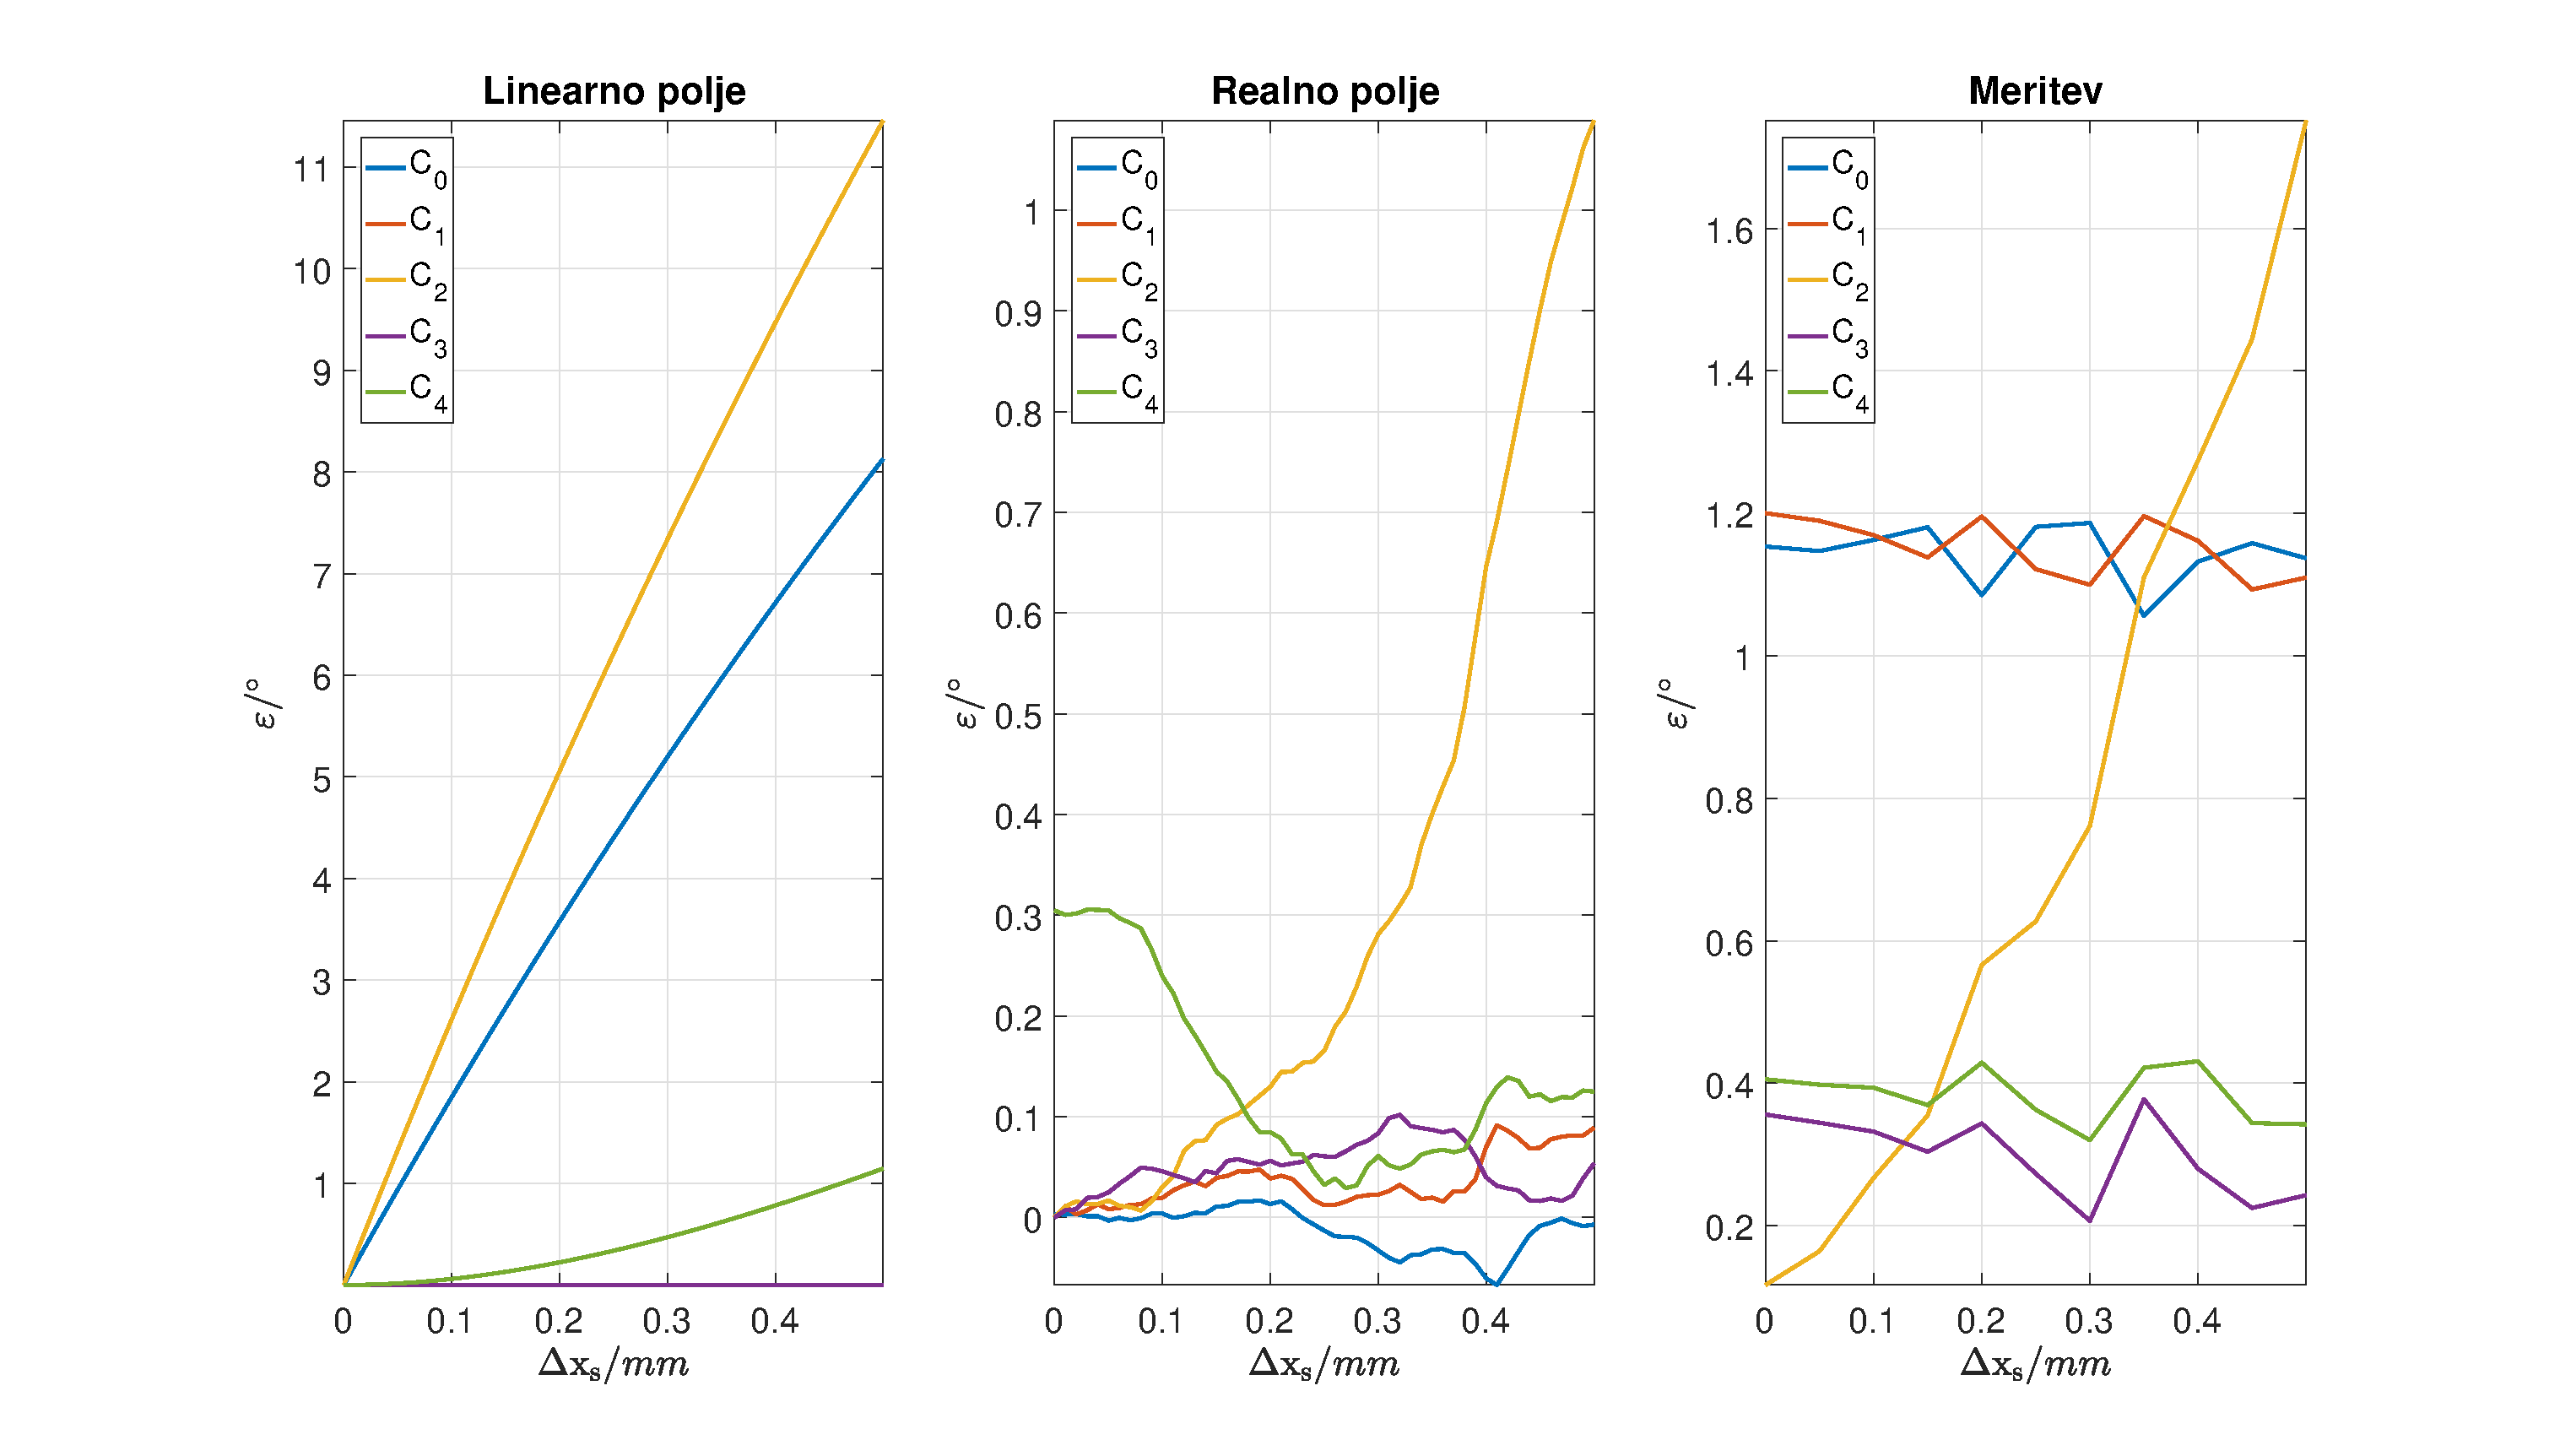
\includegraphics[width=\columnwidth]{./Slike/primerjava_xs.eps}
	\caption{Primerjave potekov amplitud harmonikov napake  statične ekscentričnosti v smeri x}
	\label{primerjava_xs}
\end{figure}
\section{Statična ekscentričnost v smeri y}
Rezultati statične ekscentričnosti v smeri y so predstavljeni na sliki \ref{primerjava_ys}. Simulacijski model z dvema sondama in linearno Z-komponento gostote magnetnega polja je pri statični ekscentričnosti v smeri y napovedoval negativno enosmerno komponento. Potek drugega harmonika je enak kot je bil simuliran pri statični ekscentričnosti v smeri x. Model s 4 sondami je v simulacijah prikazal  enake poteke amplitud posameznega harmonika napake, kot so bili posimulirani v smeri x. To je na nek način pričakovano, saj se napaka pri izmiku v smeri x in y po amplitudi nebi smela razlikovati. Enosmerna komponenta je zanemarljiva.

Meritve so pokazale drugačen potek drugega harmonika, ne po obliki naraščanja temveč po velikosti. Senzor ni bil postavljen v pravilno izhodiščno lego, saj je z opremo ki je bila na voljo ni bilo mogoče določiti. Znotraj senzorja, na čipu AM256 je pin Error, s katerim si uporabnik lahko pomaga najti izhodiščno lego. Senzor, tega pina nima na voljo zato je bila izhodiiščna lega iskana na podlagi analognih signalov $B_{sin}$ in $B_{cos}$ ter napake. Rezultati meritev prikazani na sliki \ref{primerjava_ys}, a z zavedanjem da bi morala biti amplituda drugega harmonika nižja. Potek amplitude prvega harmonika in enosmerne komponente je dokaj konstanten, kar nakazuje na neodvisnost od statične ekscentričnosti.

Pri statični ekscentričnosti so simulacije z dvema sondama podale osnovne trende napake. Simulacije statične ekscentričnosti z realnim poljem so se dobro približale končnim meritvam.
\begin{figure}[ht]

	\centering
	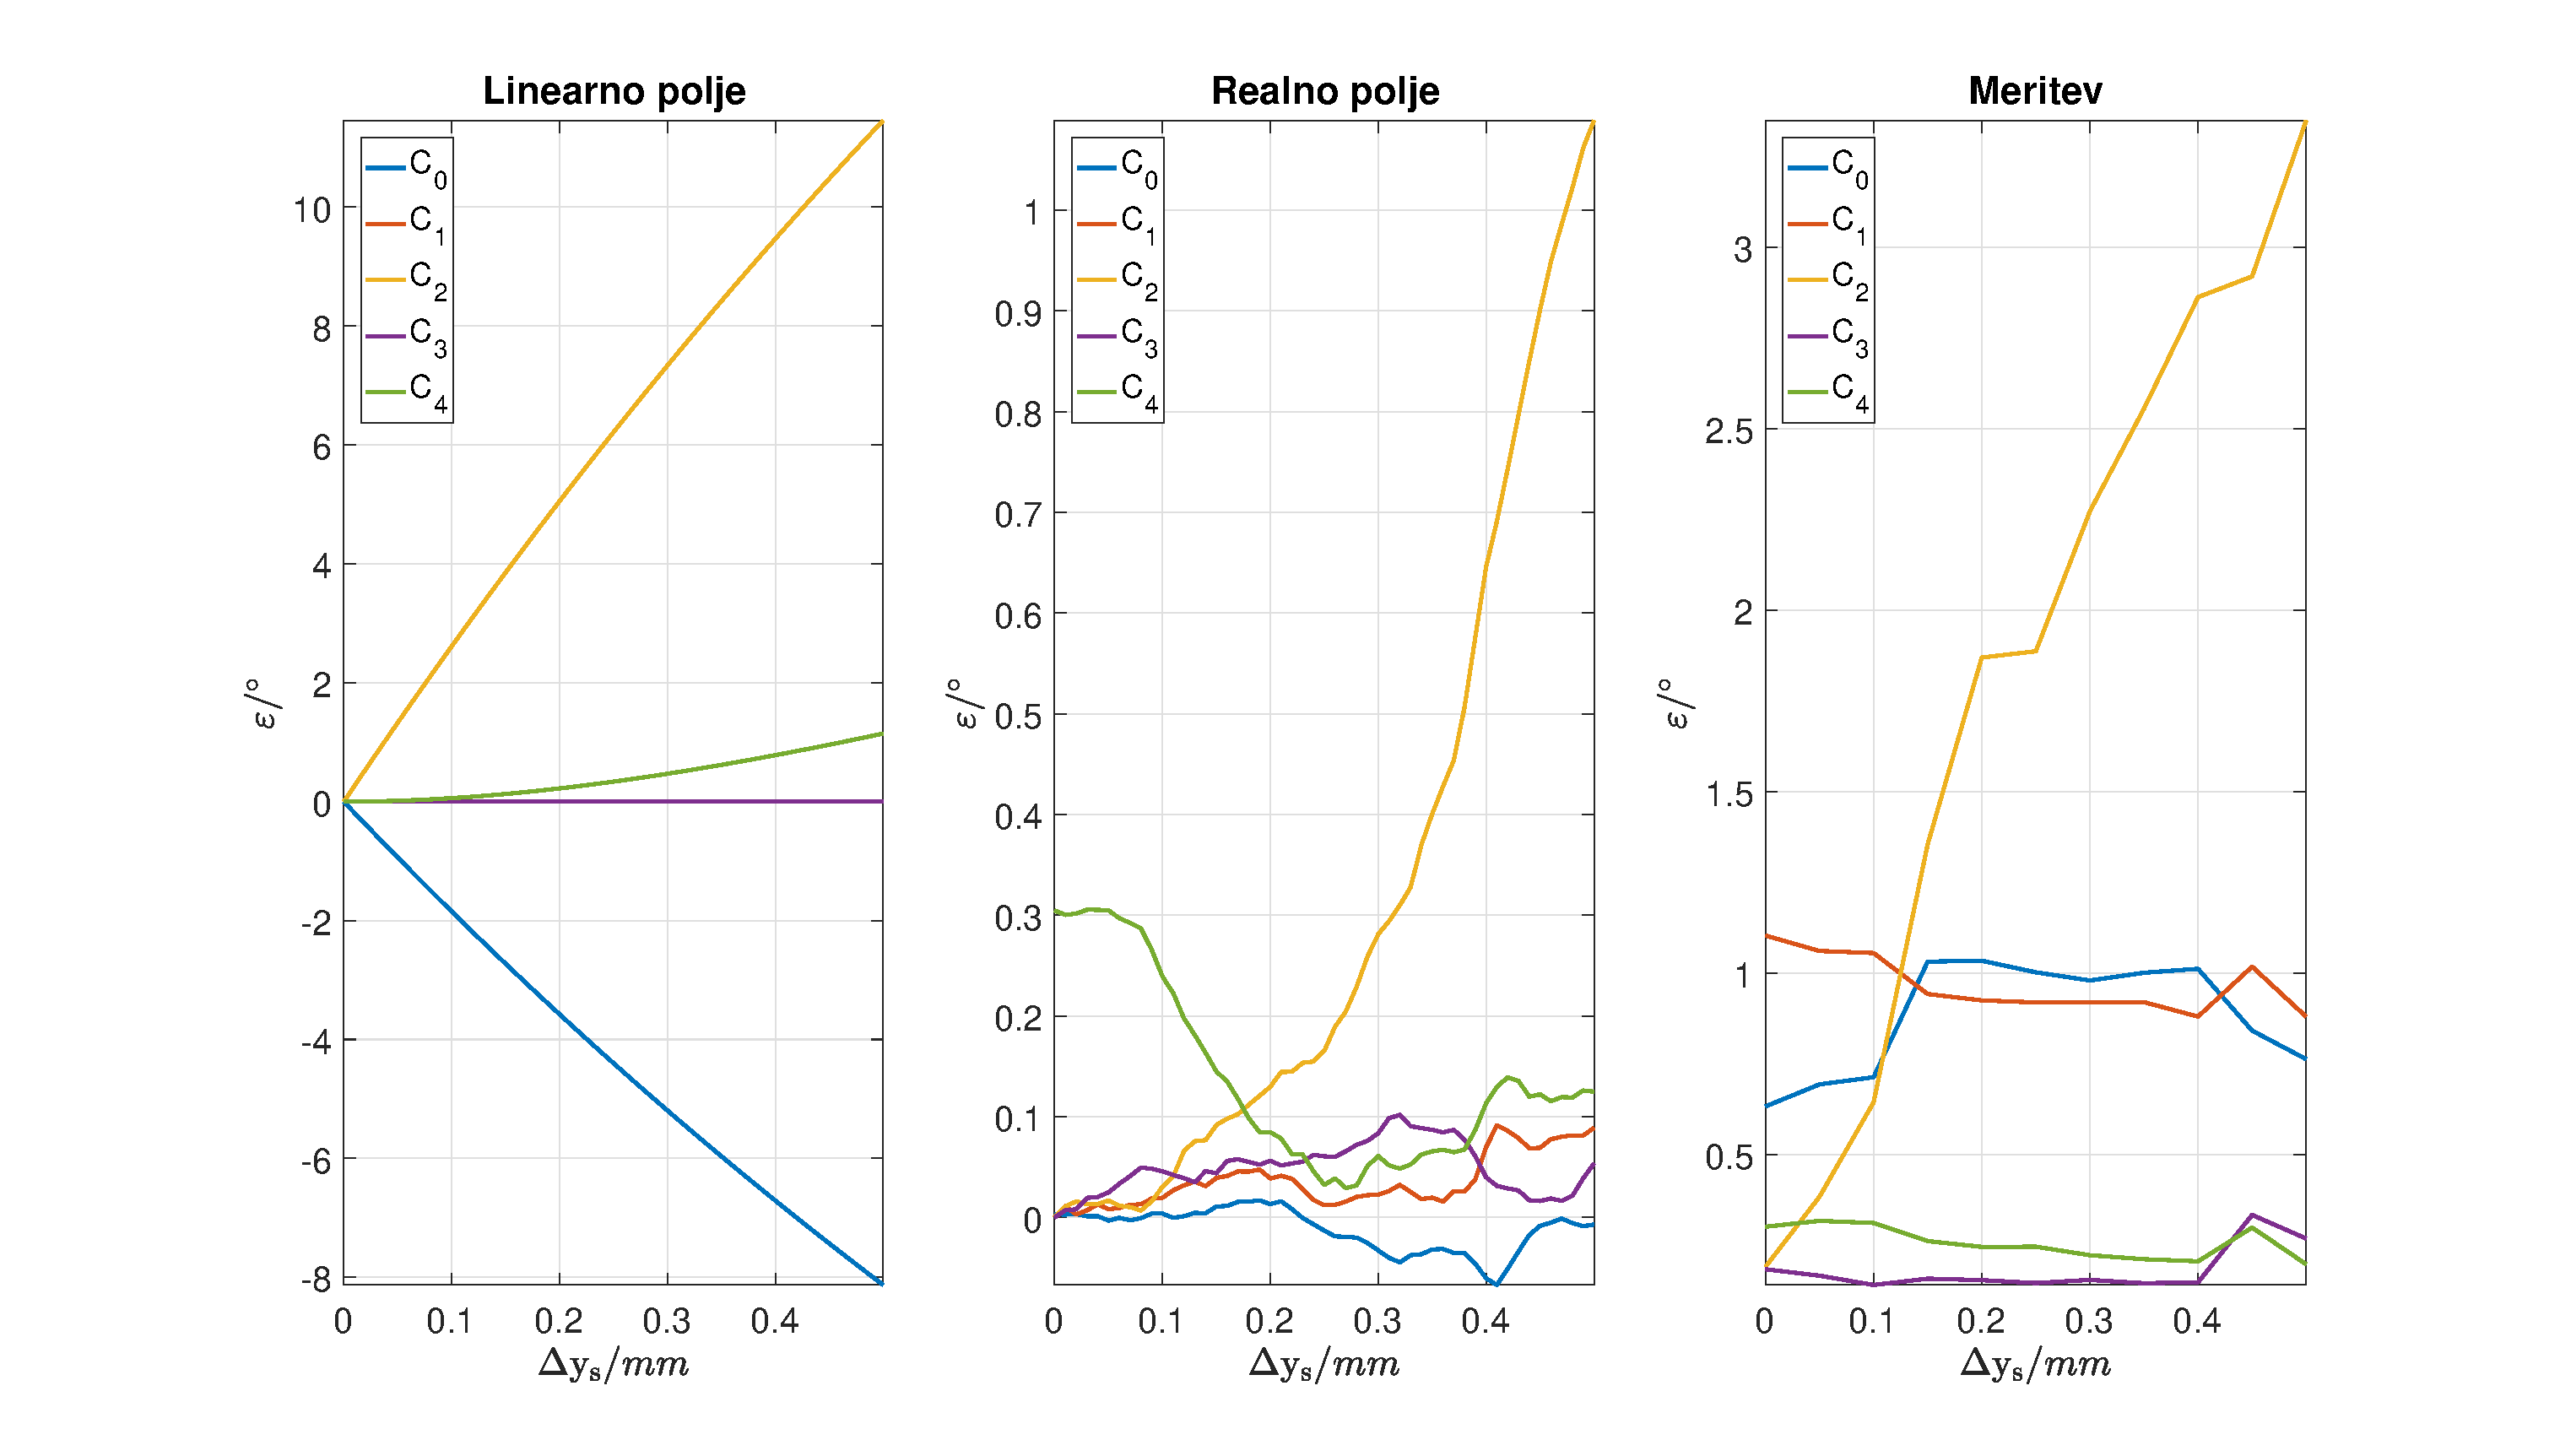
\includegraphics[width=\columnwidth]{./Slike/primerjava_ys.eps}
	\caption{Primerjave potekov amplitud harmonikov napake  statične ekscentričnosti v smeri y}
	\label{primerjava_ys}
\end{figure}

\section{Dinamična ekscentričnost}
Rezultati dinamične ekscentričnosti v smeri x so predstavljeni na sliki \ref{primerjava_xd}. Dinamična ekscentričnost je vpliva na enosmerno komponento siganal, ki ga zajame sonda. V simulacijah z dvema sondama in linearnim poljem je zato v napaki naraščal prvi harmonik napake. V simulacijah s 4 sondami in diferencialnim merjenjem  se je enosmerno komponento v $B_{sin}$ in $B_{cos}$ izničilo. V napaki se je spreminjala  enosmerna komponenta. Razlog zato je nova začetna točka.

Enosmerna komponenta se je v meritvah izrazila očitnejše, kar ni bilo pričakovano. Ostali harmoniki so ohranili svojo vrednost.

Simulacije dinamične ekscentričnosti končnih meritev ne opišejo dovolj zadovoljivo.
\begin{figure}[ht]
	\centering
	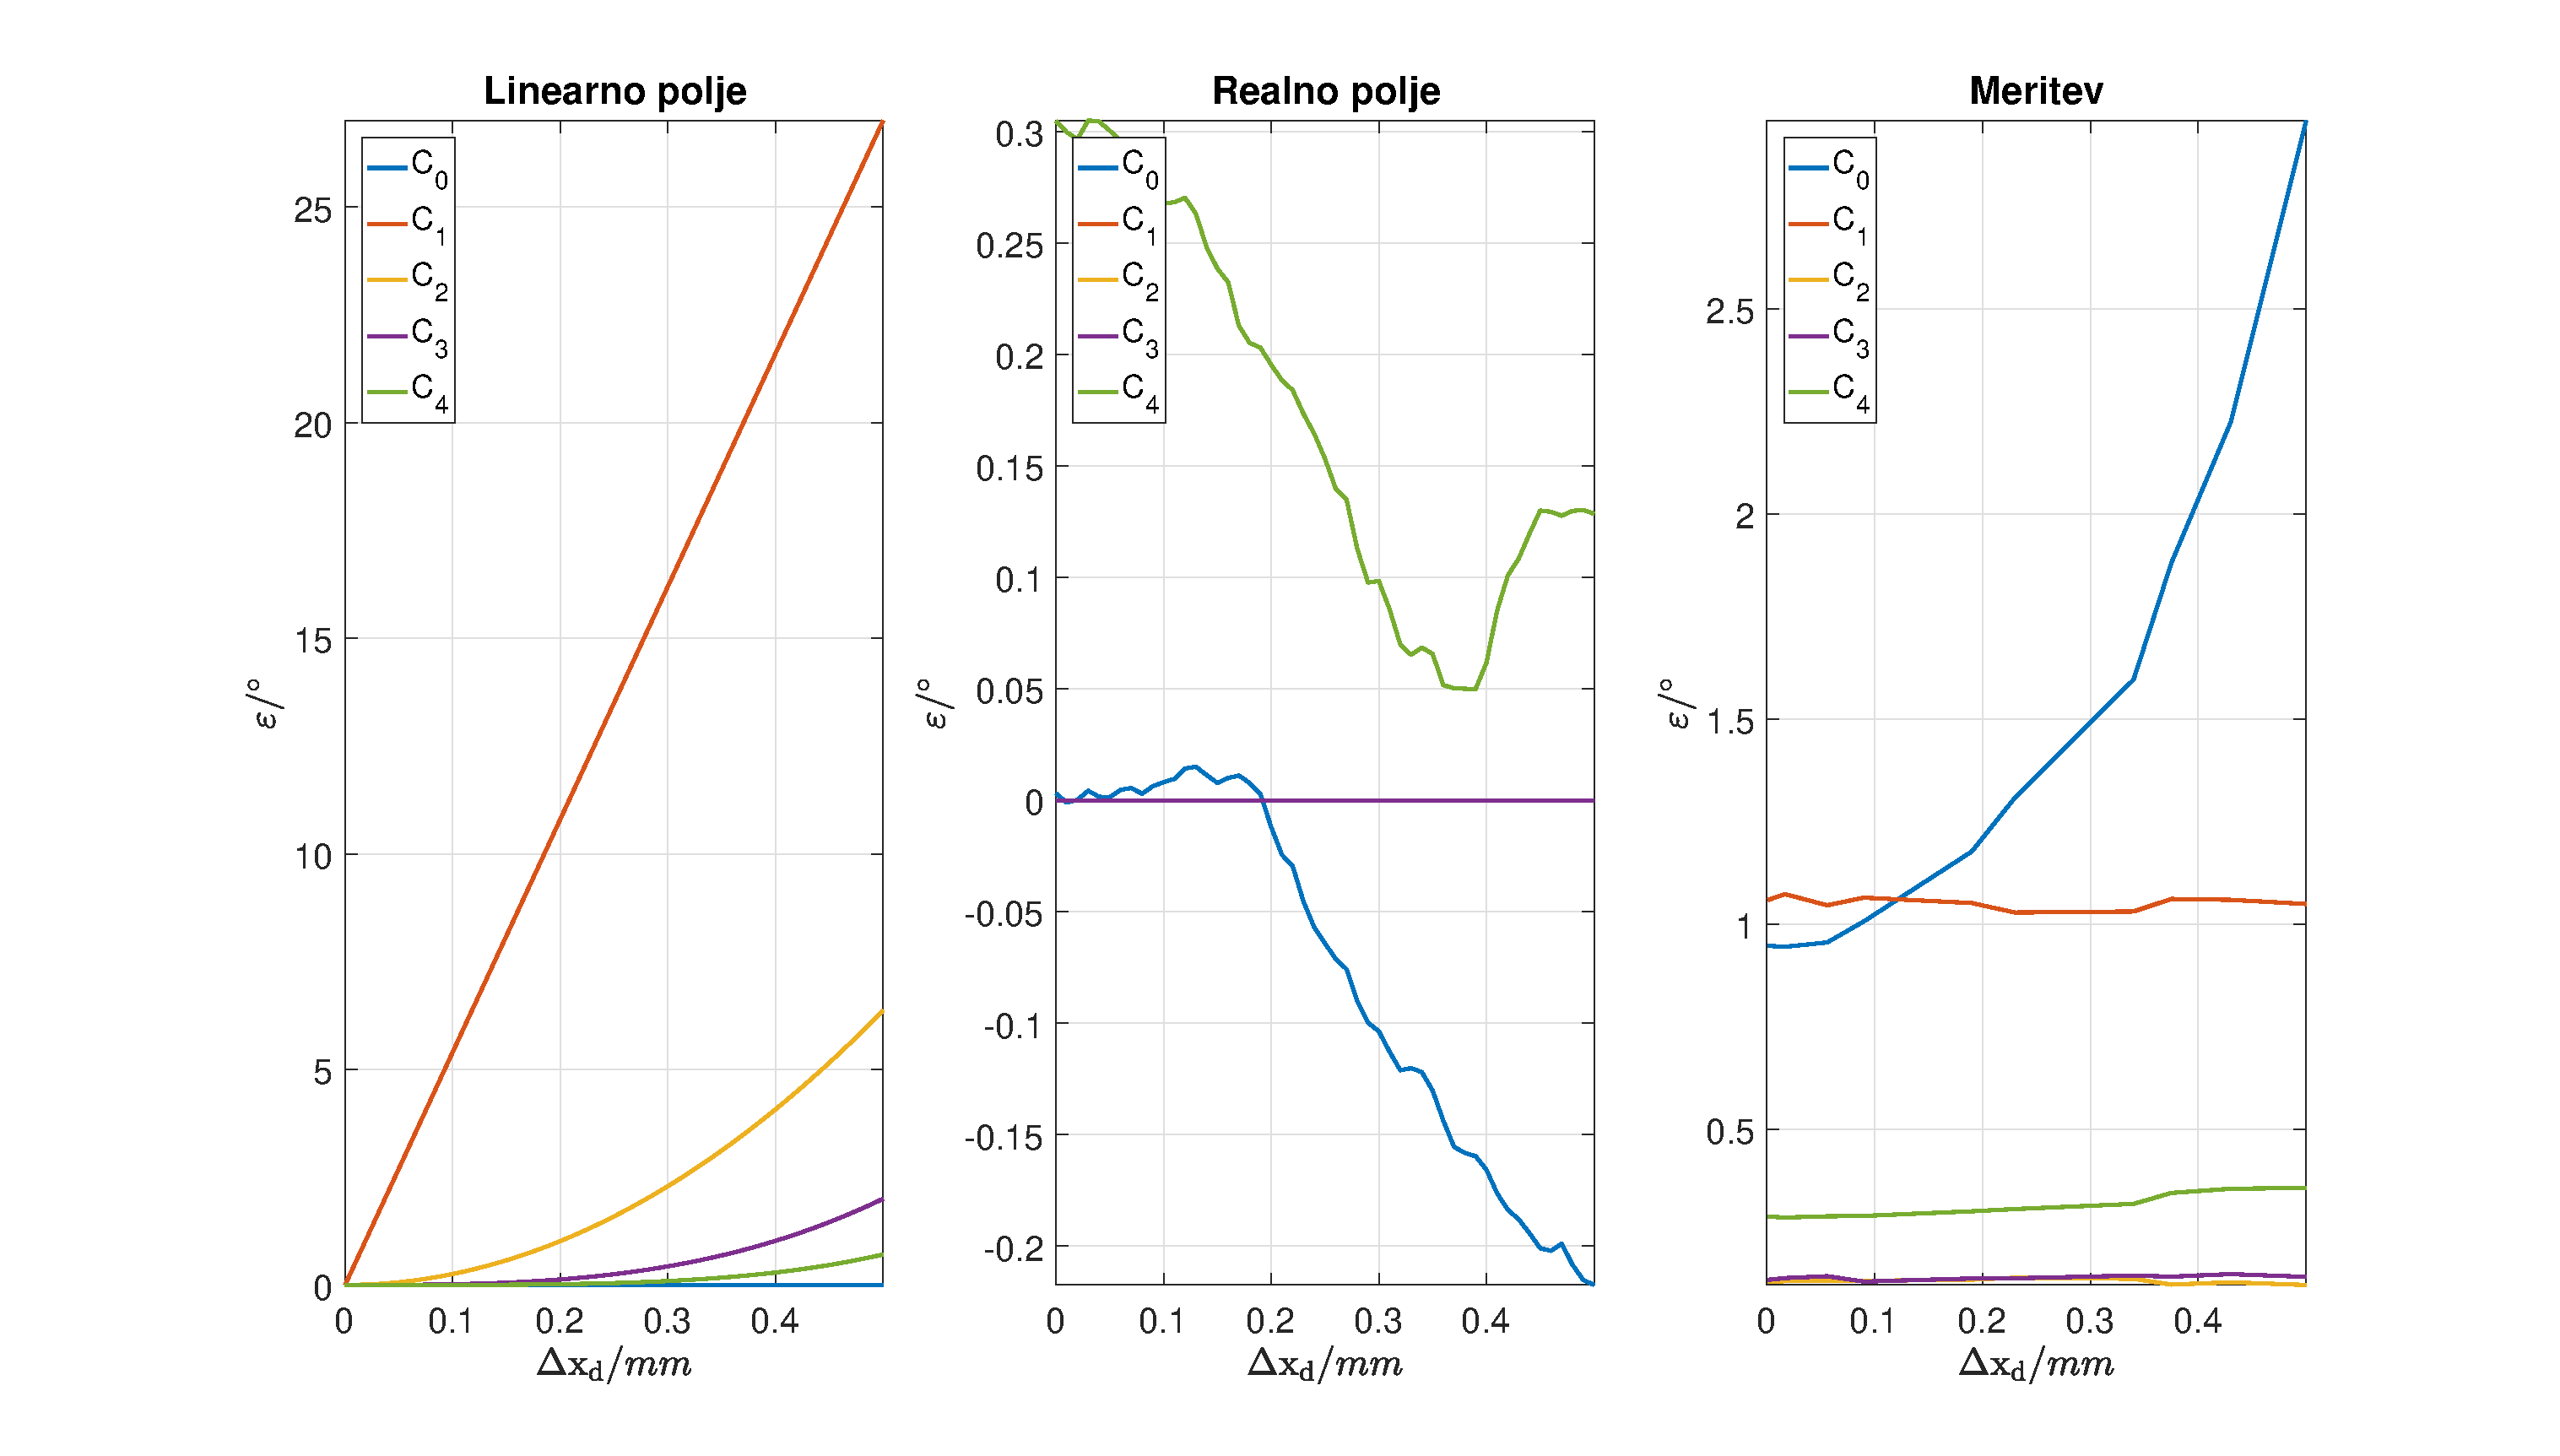
\includegraphics[width=\columnwidth]{./Slike/primerjava_xd.eps}
	\caption{Primerjave potekov amplitud harmonikov napake  dinamične ekscentričnosti v smeri x}
	\label{primerjava_xd}
\end{figure}
